%2025 - 3a
\section{03a Chapitre 2 : Variétés différentielles (suite)}

Rappel : topologie, voisinage, limite, continuité

\subsection{variété topologique}
Une variété topologique de dimension n est un espace topologique $(\mc{M}, \mc{O})$ que l'on peut cartographier autour de chaque point :

\[
\forall p \in \mc{M}, \exists \mc{U} \in \mc{O}, p \in \mc{U} et \exists une\ application x : \mc{U} \to \mb{R}\ telle\ que\ x\ soit\ continue,\ inversible\ et\ x^{-1}\ continue
\]

$\mb{R}$ muni de la topologie standard (engendré par les boules ouvertes)

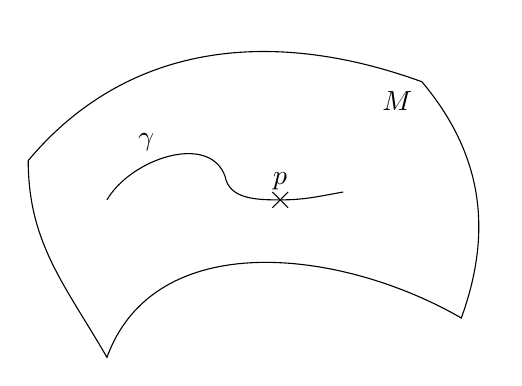
\begin{tikzpicture}
\draw(-3, 1) to[out=50, in=160] (2,2) node[below left]{$M$}
to[out=-50, in=70] (2.5,-1)
to[out=150, in=70] (-2,-1.5)
to[out=120, in=-90] (-3, 1); % Espace
%
\draw(-1.5,1) node[above]{$\gamma 	$};
\draw(-2,0.5) to[out=60, in=110] (-0.5,0.8)
to[out=-80, in=180]  (0.2,0.5) node[above]{$p$}
to[out=0, in=190] (1,0.6); % Courbe
%
\draw(0.1,0.6) -- (0.3,0.4);
\draw(0.1,0.4) -- (0.3,0.6);
\end{tikzpicture}
\subsection{Notion d'homéomorphisme}
Un homéomorphisme entre deux espaces topologiques est une bijection continue d'inverse continue

 =  Deux ensembles homéomorphe sont le même du point de vues de la topologie.

Courbe sur un espace topologique

Variété topologique de dimension n : cartes, atlas

Variété différentielle

- cartes C\_k compatibles, atlas C\_k

- variété lisse

- structure différentielle


